\documentclass[10pt,conference]{IEEEtran}
\usepackage[utf8]{inputenc}
\usepackage{amsmath}
\usepackage{amsfonts}
\usepackage{amssymb}
\usepackage{graphicx}
\usepackage{cleveref}
\usepackage{relsize}

%% EDITING
\newcommand{\ie}{i.e.\ }
\newcommand{\eg}{e.g.\ }
\crefname{section}{\S}{\S\S}
\crefname{subsection}{\S}{\S\S}
\crefname{subsubsection}{\S}{\S\S}
\crefname{equation}{}{}

%% MATHS
\newcommand{\round}{\mathrm{Round}}
\newcommand{\pfp}{+_{\mathrm{fp}}}
\newcommand{\absv}[1]{\vert #1\vert}
\newcommand{\Pro}{\mathbb{P}}
\newcommand{\F}{\mathbb{F}}
\newcommand{\R}{\mathbb{R}}
\newcommand{\ceil}[1]{\lceil #1 \rceil}
\newcommand{\floor}[1]{\lfloor #1 \rfloor}
\newcommand{\intvl}[1]{\mathlarger{\left[\right.}  #1 \mathlarger{\left.\right]}}
\newcommand{\inv}{^{-1}}
\newcommand{\fintvl}[1][x]{\mathlarger{\lfloor}#1,#1\mathlarger{\rceil}}
% Machine operation
\newcommand{\mop}{\mathtt{op_m}}
% Infinite-precision operation
\newcommand{\iop}{\mathrm{op}}
% Expectation
\newcommand{\Exp}[1]{\mathbb{E}\left[#1\right]}


\title{A probabilistic approach to the accuracy and stability of numerical algorithms}
\author{George Constantinides and Fredrik Dahlqvist \\ Department of Electrical and Electronic Engineering\\ Imperial College London}
\begin{document}
\maketitle

\begin{abstract}

\end{abstract}

\section{Introduction}

IEEE arithmetic \cite{ieee754} is traditionally modelled mathematically as follows \cite{higham2002accuracy}: if $x,y$ are two floating-point representable numbers and $\iop\in\{+,-,\times,\div\}$ is an infinite-precision arithmetic operation, then the floating-point precision implementation $\mop$ of $\iop$ must satisfy:
\begin{align}
x~\mop~y=(x~\iop~y)(1+\delta), \qquad\absv{\delta}\leq u\label{eq:traditional}
\end{align}
where $u$ is the unit roundoff for the given precision. \cref{eq:traditional} says that the machine implementation of an arithmetic operation can make a \emph{relative error} of size $\delta$ \emph{for some} $\delta\in\left[-u,u\right]$. The `\emph{for some}' is essential: this is a \emph{non-deterministic model}, we have no control whatsoever over which $\delta$ appears in \cref{eq:traditional}. This means that numerical analysis based on this model \emph{must} consider \emph{all} possible values $\delta$, \ie numerical analysis based on \cref{eq:traditional} is fundamentally a \emph{worst-case analysis}. 

It also follows from the perspective of \cref{eq:traditional} that any program doing arithmetic is, in fact, a non-deterministic program. Moreover, since the output of such a program might very well turn out to be the input of another program doing arithmetic, one should also consider non-deterministic inputs. This is precisely what happens in practice with tools for numerical analysis like Daisy \cite{darulova2018daisy} or FPTaylor \cite{solovyev2018rigorous} which require for each variable of the program a range of possible values in order to perform a worst-case analysis.

For a wide variety of programs however, it makes sense to assume that the inputs are \emph{probabilistic} rather than non-deterministic; that is to say we have some statistical model of the inputs of the program. This situation is in fact incredibly common. The inputs of one numerical routine are frequently generated randomly by another numerical routine, for example in a gradient descent optimization, a Bayesian inference algorithm, or a stochastic ray tracing algorithm. Similarly, sensors on a cyber-physical system can feed analog signals which are very well modelled statistically, to a numerical program processing these signals. 

If the inputs of a program have a known distribution, then it becomes possible, at least in principle, to ask the question: \textit{How likely are the inputs generating the worst-case rounding errors obtained from the non-deterministic model of \cref{eq:traditional}?} Typically, these inputs will occur very infrequently, and in this respect the non-deterministic model can be overly pessimistic since worst-case behaviours might in practice be such rare events that they are never encountered. 

In this paper we will explore a quantitative model which formally looks very similar to \cref{eq:traditional}, namely
\begin{align}
x~\mop~y=(x~\iop~y)(1+\delta), \qquad\delta\sim dist \label{eq:probabilistic}
\end{align}
but now $\delta$ is \emph{sampled} from $dist$, a probability distribution whose support is $\left[-u,u\right]$. In other words we move from a non-deterministic model of rounding errors to a \emph{probabilistic} model of rounding errors. This model will allow us to formalise and answer questions like \textit{What is the average rounding error?} \textit{What is the worst-case error with $99.9\%$ accuracy?}

Note that whilst in the perspective of \eqref{eq:traditional} any numerical program is a non-deterministic program, in the perspective of \cref{eq:probabilistic} every numerical program is a \emph{probabilistic program}. The study of probabilistic programs goes back to Kozen \cite{K81c}, and indeed the way in which we will understand how programs process the randomness generated by rounding errors follows precisely from the framework laid out in \cite{K81c}. (A WORD TO THE EFFECT THAT PROBABILISTIC PROGRAMS ARE A HOT TOPIC FOR THE MOMENT?)

The probabilistic model \cref{eq:probabilistic} is not new, it can be traced back to von Neumann and Goldstine \cite{von1947numerical} and is very similar to the so-called Monte-Carlo arithmetic of \cite{parker1997monte}. More recently, the model \cref{eq:probabilistic} has been investigated by Higham \cite{higham2019new}
and Ipsen \cite{ipsen2019probabilistic}. Interestingly, because \cite{higham2019new,ipsen2019probabilistic} are interested in large-dimensional problems, neither work needs to explicitly specify the distribution $dist$ for the random variable representing the relative rounding error in \cref{eq:probabilistic}. Instead, \cite{higham2019new} requires that each sample from $dist$ be independent and that $\Exp{\delta}=0$, whilst \cite{ipsen2019probabilistic} just requires that $\Exp{\delta}=0$. By using concentration of measure inequalities the authors then obtain probabilistic bounds which are independent of any particular choice of distribution. 
These bounds however are only useful for large programs. Here we will derive a principled distribution $dist$ for the relative error $\delta$ in order to apply the probabilistic model \cref{eq:probabilistic} to small to medium programs, in particular some benchmark from the literature on verification of numerical programs.

\section{A probabilistic model of rounding errors}

\subsection{Rounding error distribution}\label{subsec:error_dist}

\begin{itemize}
\item Compute the distribution of the random variable $\frac{X-\round(X)}{X}$ given the random variable $X$
\item Show that under mild assumptions on the distribution of $X$, the distribution of rounding errors is given by the roughly trapezoidal distribution of Fig \ref{fig:trapeze}.
\begin{figure}[ht!]
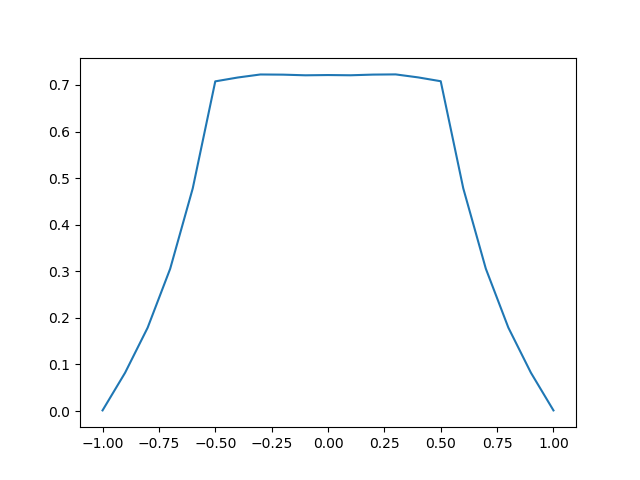
\includegraphics[scale=0.55]{trapeze_dist}
\caption{Typical distribution of rounding errors (in unit roundoffs)}
\label{fig:trapeze}
\end{figure}
\end{itemize}


\subsubsection{Derivation of the rounding error distribution}
Suppose a continuous (real-valued) random variable $X$ is distributed according to a probability density function $f$ (for example $X$ could model a stochastic, analog input signal), we can explicitly compute the distribution of the relative error induced by the quantization procedure (for example when the analog signal is digitized). We will `normalize' the result by working in units of $u$, the unit roundoff. Since the relative rounding error lies in the interval $[-u,u]$, the normalized relative error will lie in the interval $[-1,1]$.  We start by looking at the cumulative distribution function, \ie we compute the function:
\begin{align*}
c(t):=\Pro\left(\frac{X-\round(X)}{X}\leq tu\right)
\end{align*}
where $u$ is the unit roundoff. Clearly $\round(X)$ can take any value in $\F$, and given $x\in\F$ it is only possible to have $\round(X)=x$ if $X\in \left[\floor{x},\ceil{x}\right[$. This partitions $\R$

\subsection{Probabilistic version of the IEEE 754 standard}\label{subsec:prob_ieee754}

\begin{itemize}
\item Replace the usual non-deterministic 
\[
x\pfp y=(x+y)(1+\varepsilon), \absv{\varepsilon}\leq u
\]
with
\[
x\pfp y=(x+y)(1+\varepsilon)
\]
where $\varepsilon$ is a random variable of known distribution.
\item The `typical' distribution of $\varepsilon$ is described in \cref{subsec:error_dist}.
\end{itemize}

\section{Rounding error distribution of simple programs}

\subsection{Probabilistic programs}
\begin{itemize}
\item What they are: (1) programs which can sample from known probability distributions, (2) Programs whose inputs can be probabilistic.
\item The probabilistic model of IEEE 754 of \cref{subsec:prob_ieee754} turns any deterministic program into a probabilistic one.
\end{itemize}

\subsection{How probabilistic programs process probabilistic inputs}
\begin{itemize}
\item Pushing a distribution through a deterministic function
\item Pushing a distribution through a probabilistic function
\item Pushing a distribution through an \texttt{if then else} statement
\item Pushing a distribution through a simple program
\item Application to programs with probabilistic rounding errors (\cref{subsec:prob_ieee754})
\end{itemize}

\section{Probabilistic accuracy and stability}

\subsection{Accuracy: scalar products}

\begin{itemize}
\item Probabilistic accuracy
\item Comparison with classical worst-case analysis (\cite[3.1]{higham2002accuracy})
\end{itemize}

\subsection{Stability: ray tracing via the slabs method}

\bibliographystyle{plain}
\bibliography{bib/constantinides-dahlqvist}

\end{document}